\part{Introducción}

\chapter{Motivación}
\label{chapter:introduccion}

\section{Evaluaciones y opiniones}
\label{section:evaluaciones-cruzadas}

\subsection{Ítem}
\noindent Llamaremos ítem a un elemento del mundo real que es aprovechado por las personas, dicho ítem puede ser un objeto, un servicio, una idea, un programa, etc. Además, debe poder ser abstraído a un modelo representado por una computadora, de manera tal que esa representación describa con precisión a qué se refiere ante la interpretación del lector. 

\noindent Para ello, el modelo del ítem contendrá un conjunto de atributos que lo describen. Algunos más importantes que otros.
\\\\
Por ejemplo, imaginemos que se debe representar una bicicleta mediante un conjunto de pares atributo;valor, podría utilizarse una representación como la siguiente:
\begin{lstlisting}[frame=single] 
Tipo: Bicicleta
Sexo: Unisex
Talle: 51
Cuadro-Material: Aluminio
Cuadro-color: Rojo
Cuadro-Tipo: Ruta
Horquilla-Material: Fibra de carbono
Horquilla-Color: Rojo
Asiento-tipo: Adamo 
Asiento-Color: Blanco
\end{lstlisting}
La cantidad de atributos que pueden utilizarse para describir el ítem puede ampliarse prácticamente hasta el cansancio. 
\\\\\\
Reducir la cantidad de pares de atributos para describir el mismo ítem es posible de la siguiente manera: 
\begin{lstlisting}[frame=single] 
Tipo: Bicicleta
Talle: 51 
Marca: Merida
Modelo: Reacto 500
\end{lstlisting}
En este caso se aprovechó el hecho de que ya existan definiciones del ítem que intentamos describir, por lo que si se utilizan sólo los atributos que lo identifican, será suficiente para que el lector tenga la interpretación correcta del mismo. 
\\\\
\subsection{Usuario}
Las personas cotidianamente hacen uso de estos ítems, convirtiéndolos en usuarios del mismo. Y estos usuarios pueden de la misma manera ser computacionalmente representados mediante pares de atributo;valor. Y al igual que los ítems algunos atributos servirán para identificar al usuario. 
\\\\
\subsection{Reseña}
Definiremos a una reseña (de aquí en adelante review) a la representación mediante la computadora, de la medida de conformidad con respecto a dicha relación entre usuario e ítem. 

Esta relación de uso entre usuario e ítem que puede observarse en la figura \ref{figure:reviewItemUser}, contiene un grado de conformidad entre el primero y el segundo, si el ítem cumplió o no con las expectativas del usuario debería poder modelarse también para ser representado computacionalmente.

El objetivo de un review, es que un usuario pueda reflejar el sentimiento que le generó utilizar el ítem e informarlo a otros usuarios. 

También los reviews dispondrán de un conjunto de atributos de los cuales algunos serán indispensables y otros que enriquecerán no sólo su valor intrínseco, sino también su utilidad para el contexto en el que será planteado.
\\\\
Imaginemos un usuario que realiza un review sobre la bicicleta, podría generar el siguiente conjunto de pares atributo-valor:
\begin{lstlisting}[frame=single] 
Puntuacion:4 
Titulo:``Buena opcion''
Texto:``Liviana y comoda, pero un poco rigida para 
        doblar, y no frena adecuadamente ''
Fecha:15/10/2012
\end{lstlisting}
\begin{figure}
    \centering
    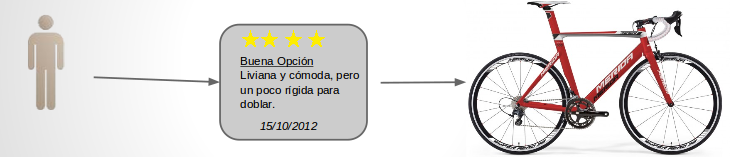
\includegraphics[width=0.8\textwidth,natwidth=610,natheight=642]{biciReview.png}
    \caption{Relación entre usuario, review e ítem}
    \label{figure:reviewItemUser}
\end{figure}

La existencia de los reviews en la web es muy importante, ya que dan un panorama socialmente perfeccionado (dado que permiten que no sólo una persona
opine sobre un ítem, lo que da a lugar a muchas evaluaciones y provoca que se acerque al valor real) sobre un ítem, característica que ayuda a 
quienes necesiten una descripción y valoración de los mismos que no provenga de quien los quiere promocionar.

\section{Sistemas de Recomendación}
\label{section:sistemas-de-recomendacion}
\noindent Los sistemas de recomendación son herramientas de software que, en base a un conjunto de ítems (películas, libros, productos, hoteles, etc) e información sobre estos, y un conjunto de usuarios, intentan sugerir ítems apropiados a dichos usuarios \cite{Systems2011}. Puede verse en la figura \ref{figure:flujo} cómo estos se componen. Los sistemas de recomendación se han vuelto una de las herramientas más poderosas para múltiples tipos de aplicaciones web, como comercio electrónico o páginas de noticias. 
\\\\
El desarrollo de estas herramientas, involucra conocimiento en múltiples áreas, como inteligencia artificial, minería de datos, estadística, etc. 
\\\\
Los sistemas de recomendación poseen tres enfoques, el de filtrado colaborativo, el basado en contenido y el no personalizado.


\begin{figure}
    \centering
    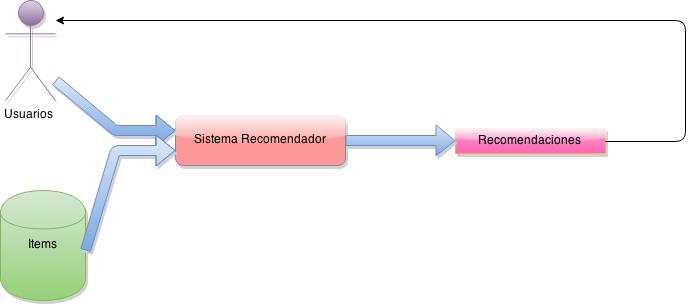
\includegraphics[width=0.8\textwidth,natwidth=610,natheight=642]{recSis}
    \caption{Flujo de un Sistema de Recomendación}
    \label{figure:flujo}
\end{figure}

\subsection{Sistemas de recomendación basados en contenido}
Los sistemas de recomendación basados en contenido utilizan un conjunto de informaciones y descripciones de los ítems previamente valorados por un usuario para poder construir un perfil del mismo de manera tal de poder determinar, cuales son sus intereses  \cite{Systems2011}.

Una vez construido el perfil, pueden procesarse las características de distintos ítems que potencialmente pueden ser recomendados a dicho usuario para determinar si alguno de ellos va acorde al perfil.
\subsection{Sistemas de recomendación de filtrado colaborativo}
Los sistemas de recomendación de filtrado colaborativo utilizan la información histórica de cada usuario para intentar encontrar y generar grupos de usuarios con gustos similares \cite{Systems2011}. Para lograrlo se compara cada usuario con otro observando qué ítems evaluaron y qué puntajes fueron otorgados. 

De esta forma, si se requiere predecir el interés de un usuario en un ítem, se podrá buscar en dicho grupo de usuarios con gustos similares e inspeccionar aquellos usuarios que hayan realizado un review sobre el ítem.
\\\\
Los sistemas de recomendación de filtrado colaborativo tienen una eficacia superior a los basados en contenido, pero cuentan con una gran desventaja, no permiten predecir intereses para aquellos ítems que aún no poseen evaluaciones, o también para aquellos usuarios que no han evaluado ningún ítem.  A esto se lo llama “arranque en frío”.
\subsection{Sistemas de recomendación no personalizados}

Éste es el más simple de los sistemas de recomendación, ya que como refiere su nombre, no 
toma en cuenta las características de los usuarios.\\
Su funcionalidad se basa en el background de información obtenida sobre los ítems, recomendándolos
indistintamente a cada uno de los usuarios habiendo previamente generado un ranking de popularidad \cite{Poriya2014}.
Opcionalmente puede generarse más de un ranking separando los tipos de ítems (Por ejemplo tener un ranking de 
películas y otro de libros).\\
\\
Estos sistemas de recomendación son muy populares entre los eCommerce.
\section{La web semántica}
\label{section:la-web-semantica}
En sus comienzos en los 90, la web podía verse como un conjunto de sitios web que ofrecían una colección de documentos web interconectados mediante la hipermedia, con el objetivo de comunicar información a los usuarios.
El contenido de esos documentos sólo era generado por el mismo creador y publicador del documento y los usuarios se limitaban a consumirlo. Por otro lado, era a su vez estático, es decir, se publicaba en la misma forma que se almacenaba y no cambiaba.  
\\\\
Hacia fines de los 90 los sitios web comenzaron a implementar una serie de herramientas (que si bien ya se encontraban disponibles anteriormente no se utilizaban por un problema de performance) que permitieron a los usuarios finalmente participar de la producción del contenido web. Lo que produjo notorios cambios en cuanto a la cantidad de información disponible y proveyó diferentes formas de uso de la web (blogs, redes sociales, canales rss, etc). Más adelante ante la apreciación del pasaje de web estática a una web dinámica, se acuño a esa actual web como web 2.0 y retrónimamente 1.0 a la anterior.
\\\\
Ese cambio provocó un aumento en el tamaño de la web, que se volvió inmensamente grande, y llevó a la necesidad de implementar tecnologías que ayuden al aprovechamiento de esa cantidad de información. 
Se comenzó entonces a utilizar una serie de frameworks y estándares que permitieron enriquecer mediante metadatos semánticos y ontológicos dentro de los estándares de la W3C los datos contenidos en los documentos de manera tal que estos puedan ser consumidos, interpretados y utilizados directamente no sólo por las personas, sino también por las computadoras.
Esto generó que los datos también puedan ser relacionados entre sí, de la misma manera que los documentos son interconectados formando una web de documentos, los datos interconectados forman una web de datos paralela\cite{DiNoia2012}.
Todo este conjunto de actividades frameworks y herramientas forman la ``Web semántica'' que es el puntapié inicial para una web mucho más interoperable, lo que permite facilidades para el uso de la web por parte de las aplicaciones y da lugar a otro paso en la evolución de la web, la web 3.0. 
La figura \ref{figure:webevolution} muestra ejemplos de las tecnologías más importantes que marcaron cada uno de los puntos de evolución recientemente mencionados.

La Web Semántica promete facilitar el desarrollo de la web social y la inteligencia colectiva, a través de mecanismos de clasificación, relación y descripción del contenido de la información publicada mejorando su interoperabilidad \cite{Antoniou}. Promete también mejorar la recolección, agregación e integración de datos específicos mediante el uso de agentes de búsqueda automáticos que aprovechan las ventajas.
%Con el correr de los años, múltiples tecnologías se fueron implementando y permitieron el desarrollo de una web mucho más grande y aprovechable...  y esto es una referencia a un libro sobre web semántica \cite{Antoniou}

\begin{figure}
    \centering
    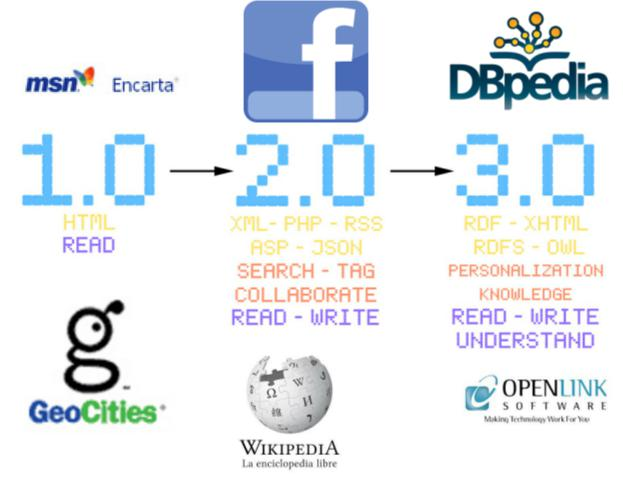
\includegraphics[width=0.8\textwidth,natwidth=610,natheight=642]{webevolve}
    \caption{Evolución de la web}
    \label{figure:webevolution}
\end{figure}

\section{Reviews en la web semántica}
\label{section:reviews-en-la-web}

La web 2.0 dio la posibilidad a los usuarios consumidores de la web de generar y publicar contenido en la misma, lo cual cumple con los requerimientos de una plataforma para reviews. Proporciona un entorno para crearlos y publicarlos, siendo está última una tarea muy sencilla. 

Pero la dificultad de encontrarlos y explotarlos parece ser inversamente proporcional a a la de generarlos. Dado que a mayor facilidad de publicar contenido en la web, mayor se vuelve la inmensidad de la misma y mayor se vuelve la dificultad de encontrar algo dentro de ella.

Veamos dos ejemplos que requieren encontrar reviews en la web y cómo la web semántica puede facilitarlo:

Imagínense que son ingenieros de Mérida y lanzaron al mercado la bicicleta Reacto 500. Como buenos ingenieros necesitan conocer qué opinan sus clientes, por lo que buscarán reviews en algún motor de búsqueda y luego leerán uno por uno cada review con el objetivo de resumir las opiniones. Humanamente realizar esta tarea para unos pocos reviews podría demandar mucho tiempo. 
Incluso peor aún, imagínense que necesitan saber que opina la gente de determinada región (por ejemplo el norte de Europa), la tarea de buscar los reviews necesarios se volvería aún más complicada.
Con la posibilidad de contar con una web en la cual los datos son interpretados por las aplicaciones de software y estos a su vez están interconectados, podría crearse una aplicación que pueda automáticamente buscar, clasificar y procesar los reviews para generar automáticamente el resumen.

Ahora bien, si en lugar de requerir reviews de un ítem en particular, se necesitan reviews para una aplicación que recomiende ítems a usuarios, ya no sería una tarea realizable humanamente. Para ello haría falta una aplicación que haga crawling en la web y de alguna manera identifique reviews y a su vez identifique el ítem al cual el review hace referencia. 
Parece algo muy difícil de lograr, aún trabajando sobre sitios conocidos con documentos estructuralmente dominados los cuales se pueda recorrer el DOM automáticamente y acceder a los reviews.
De nuevo, la Web Semántica promete solucionar este problema \cite{Heitmann}, con el uso de metadatos que dan información sobre los datos, haciendo que una aplicación pueda fácilmente identificar reviews y navegar por la hipermedia de los datos para conseguir información sobre el ítem y usuario referenciados \cite{Zhou2005}.

La figura \ref{figure:semanticwebreview} muestra un ejemplo concreto de un review publicado en la web, respetando los lineamientos de la web semántica. 

\begin{figure}
    \centering
    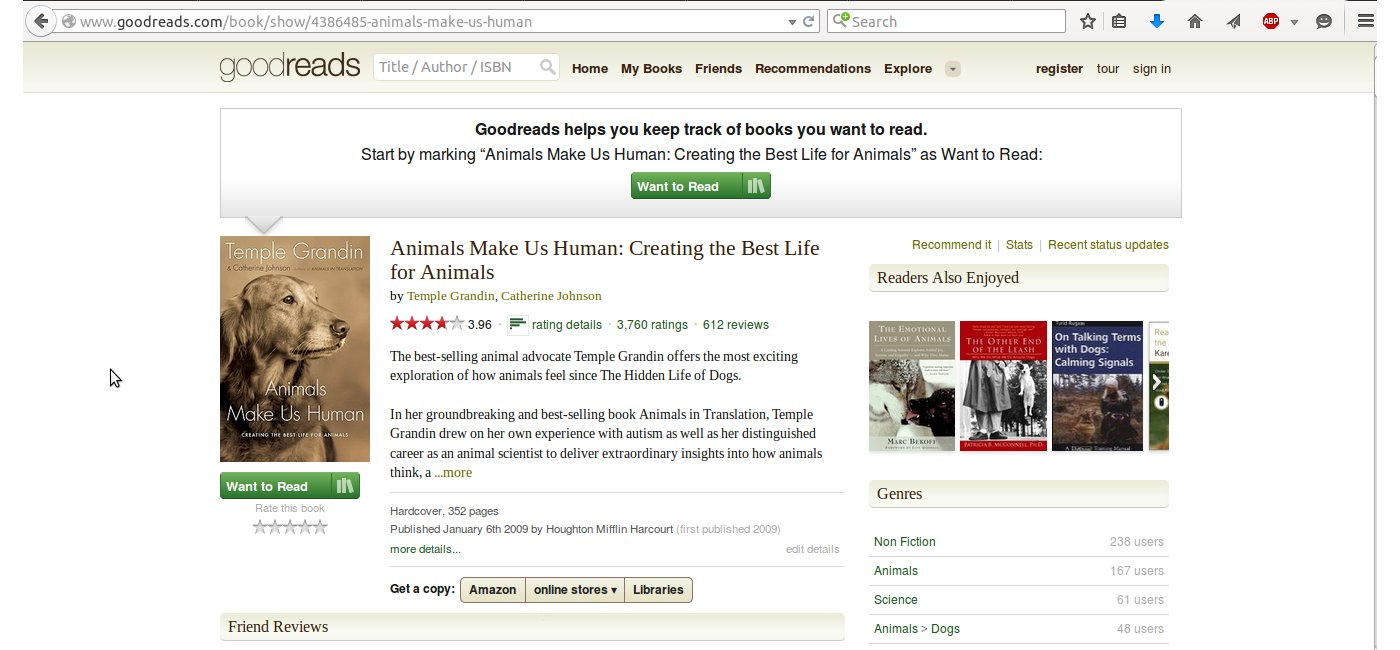
\includegraphics[width=0.8\textwidth,natwidth=610,natheight=642]{semanticwebreview}
    \caption{Ejemplo de review en la web semántica}
    \label{figure:semanticwebreview}
\end{figure}

En \cite{Heath2006} se presenta un sistema con el objetivo de publicar reviews en la web semántica. Dicho sistema no tuvo éxito
y la funcionalidad del mismo se encuentra actualmente inoperable.

\section{Caso de estudio}
\label{section:caso-de-estudio}
Para mantener en contexto este trabajo, utilizaremos un caso de estudio. Se trata de una aplicación que integra información de reviews disponible en la web semántica para producir recomendaciones simples. En particular, ofrece los siguientes servicios: 

\begin{description}
\item[Rankings de calidad ] Los rankings de calidad son listas de ítems ordenadas por el promedio de puntos 
obtenidos de sus reviews. Para construirlos en necesario obtener y combinar los puntajes de cada uno
de los reviews de cada ítem.
\item[Rankings de popularidad] Los rankings de popularidad son listas de ítems ordenadas por la cantidad
de reviews que posee cada ítem.
\item[Listas de tipos] Las listas de tipos son listas de los distintos tipos de ítem encontrados. 
Por ejemplo, películas, libros, productos, etc.
\item[Listas de ítems] Las listas de ítems son listas resultantes de búsquedas de ítems por nombre o por tipo. 
Para su construcción es necesario contar con los nombres o tipo de cada ítem.
\item[Filtro] Los filtros son opciones de filtrado de los rankings, para reducir la cantidad 
de ítems retornados por ellos. De manera que se puedan seleccionar ítems por fecha de review.
\item[Descripciones] Las descripciones son los detalles de los ítems, que incluyen toda la información que se dispone de estos 
incluyendo sus reviews. El usuario podrá recibir esta información proveyendo al sistema el id del ítem el cual se quiere consultar.
 
\end{description}


\section{Organización}
\label{section:organizacion}

 El capítulo \ref{chapter:semanticwebelements} introduce los conceptos de Web Semantica, sus principios y tecnologías y para que el capítulo \ref{chapter:estrategia} presente la estrategia de trabajo en términos generales. Los capítulos desde \ref{chapter:seleccion} a \ref{chapter:explotacion} discuten en detalle cada uno de pasos de la estrategia elegida, aplicándolos al caso de estudio. Finalmente, el capítulo \ref{chapter:conclusiones} resumen los resultados observados, saca conclusiones al respecto, y plantea trabajo futuro. El anexo \ref{anexo} presenta las publicaciones que fueron resultado del trabajo efectuado en este trabajo de tesis. 



